\documentclass[12pt,a4paper]{article}
\usepackage[MeX]{polski}
\usepackage[utf8]{inputenc}
\usepackage{listings}
\usepackage{graphicx}
\usepackage{fancyvrb}
\usepackage{tabularx}
\usepackage{geometry}
\usepackage{multirow}
\geometry{
 a4paper,
 total={170mm,257mm},
 left=20mm,
 top=20mm,
}
\author{Yurii~Vyzhha}
\title{Metody Obliczeniowe w Nauce i Technice \\ Laboratorium 1 \\
  Arytmetyka Komputerowa \\ Sprawozdanie}
\begin{document}
  \maketitle
  \paragraph{Zadanie 1 Sumowanie liczb pojedynczej precyzji}\mbox{}\vspace{3mm}\\
  \emph{Zwykły algorytm sumowania}
  \begin{Verbatim}
  float[] ar = new float[10000000];
  float v = 0.53125f;
  for (int i = 0; i < ar.length; i++) {
      ar[i] = v;
  }
  float sum = 0.0f;
  for (int i = 0; i < ar.length; i++) {
      sum += ar[i];
  }
  \end{Verbatim}
  Bezwzględny błąd: $ \sim 5.3 \%$. \\
  Względny błąd: $ 281659.5$. \\
  Wielkość błędu sumowania jest związana z reprezentacją liczb
  zmiennoprzecinkowych oraz z implementacją sumowania dwóch l.~z.
  Dla obliczenia sumy dwóch l.~z., mantysę mniejszej z liczb musimy doprowadzić
  do postaci większej z liczb co wiąże się z utratą mniej znaczących cyfr
  cechy. \\
  Poniżej przedstawiamy wykres który pokazuje zależność pomiędzy błędem
  bezwzględnym a ilością iteracji wykonanych przez program.\\
  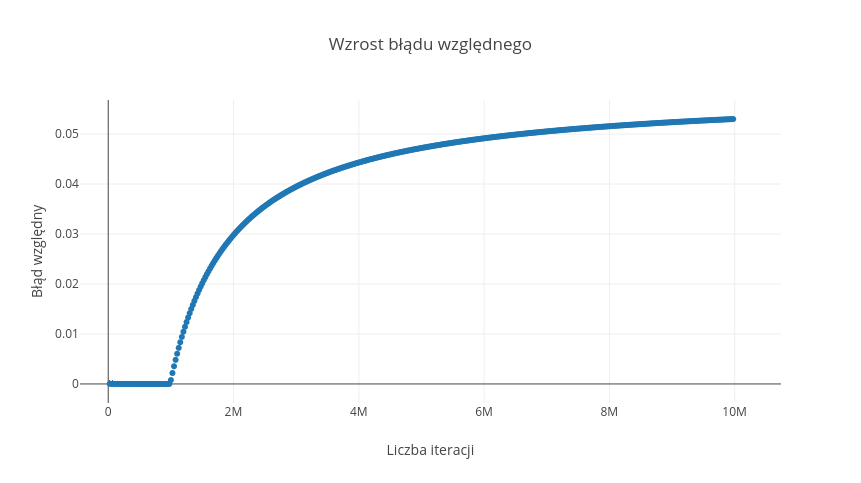
\includegraphics[width=1\textwidth]{img/Plot1} \\
  Jak widzimy na wykresie, przy pierwszych $10^6$ iteracji nie mamy błędu.
  To jest związane z tym, że wielkość cechy jest wystarczają duża, a różnica
  między liczbami, które dodajemy, jest wystarczająco mała. Później błąd
  bezwględny się pojawia, ale rośnie co raz z mniejszą prędkością. To jest
  spowodowane tym, że z każdym dodawaniem mylimy się na stałą liczbę, a suma
  rośnie, więc udział błędu w sumie jest co raz mniejszy.\vspace{3mm}\\
  \emph{Rekurencyjny algorytm dodawania}
  \begin{Verbatim}
  public static float recSum(float[] ar, int a, int b) {
      if (a == b) return ar[a];
      if (b - a == 1) {
          return ar[a] + ar[b];
      }
      return recSum(ar, a, (b + a)/2) + recSum(ar, (b + a)/2 + 1, b);
  }
  \end{Verbatim}
  Dla $v = 0.53125$: \newline
  bezwzględny błąd: $ 0.0 \% $; \newline
  względny błąd: $ 0.0 $. \newline
  Korzystając z rekurencyjnego algorytmu, przy $v = 0.53125$ nie mamy
  błędu. Ten algorytm jest zaimplementowany tak, że dodaje liczby wylącznie o
  tej samej wielkości, więc przesunięcie cechy i, co za tym idzie, utrata
  precyzji nie występują.
  \newline
  Czas działania obu algorytmów jest mniej więcej taki sam dla różnych danych
  wejściowych. \newline
  Algorytm rekurencyjny zwraca niezerowy błąd dla $v = 0.66667$. W tym przypadku,
  bezwzględny błąd jest równy $ \sim 0.000075 \% $, względny zaś $ -0.5 $.
  \paragraph{Zadanie 2 Algorytm Kahana}\mbox{}\vspace{3mm}\\
  \emph{Implementacja algorytmu Kahana w języku Java}
  \begin{Verbatim}
      float sum = 0.0f;
      float err = 0.0f;
      for (int i = 0; i < ar.length; i++) {
          float y = ar[i] - err;
          float temp = sum + y;
          err = (temp - sum) - y;
          sum = temp;
      }
  \end{Verbatim}
  Bezwzględny błąd: $ 0.0 \%$. \\
  Względny błąd: $ 0.0 $. \\
  % TODO: Wyznacz bezwzględny i względny błąd obliczeń dla tych samych danych wejściowych jak w przypadku testów z Zadania 1.
  Algorytm Kahana działa w następujący sposób. Każdego razu jak dodajemy
  nową liczbę do ogólnej sumy ($sum + y$), obliczamy korektę ($err$),
  który stosujemy w następnej iteracji. Najpierw odejmujemy korektę $err$,
  którą obliczyliśmy w poprzedniej iteracji pętli, i otrzymujemy poprawiony
  składnik $y$. Później dodajemy ten składnik do sumy $sum$. Najmniej znaczące
  bity $y$ straciliśmy przy sumowaniu. Potem obliczamy najbardziej znaczące
  bity $y$ za pomocą $temp - sum$. Kiedy odejmniemy $y$ od otrzymanej różnicy,
  odzyskamy najmniej znaczące bity. Te właśnie bity straciliśmy przy obliczaniu
  $sum + y$. One będą korektą w następnej iteracji. \newline
  Czas działania algorytmów Kahana oraz rekurencyjnego jest mniej więcej taki
  sam dla różnych danych wejściowych.
  \paragraph{Zadanie 3 Sumy częściowe}\mbox{}\vspace{3mm}\\
  Tablice nalerzy czytać w następujący sposób: najpierw podany jest wynik,
  otrzymany przy sumowaniu wprzód, a niżej w tej samej komórce wynik, otrzymany
  przy sumowaniu wstecz.\vspace{3mm}\\
  \emph{Funkcje policzone z pojedynczą precyzją:} \vspace{3mm}\\
  Funkcja dzeta Riemanna: \vspace{3mm}\newline
  \begin{tabularx}{\textwidth}{ |l|l|X|X|X|X|X| }
      \hline
      & & \multicolumn{5}{ c| }{n} \\ \hline
      & & 50 & 100 & 200 & 500 & 1000 \\ \hline
      \multirow{5}{*}{s} & 2 & 1.6251329 1.6251328 & 1.634984 1.6349839 & 1.6399467 1.6399465 & 1.642936 1.642936 & 1.6439348 1.6439345 \\ \cline{2-7}
      & 3.6667 & 1.1093994 1.1093998 & 1.1094086 1.1094089 & 1.1094086 1.1094103 & 1.1094086 1.1094105 & 1.1094086 1.1094105 \\ \cline{2-7}
      & 5 & 1.0369275 1.0369277 & 1.0369275 1.0369277 & 1.0369275 1.0369277 & 1.0369275 1.0369277 & 1.0369275 1.0369277 \\ \cline{2-7}
      & 7.2 & 1.0072277 1.0072277 & 1.0072277 1.0072277 & 1.0072277 1.0072277 & 1.0072277 1.0072277 & 1.0072277 1.0072277 \\ \cline{2-7}
      & 10 & 1.0009946 1.0009946 & 1.0009946 1.0009946 & 1.0009946 1.0009946 & 1.0009946 1.0009946 & 1.0009946 1.0009946 \\
      \hline
  \end{tabularx} \vspace{3mm}\newline
  Funkcja eta Dirichleta: \vspace{3mm}\newline
  \begin{tabularx}{\textwidth}{ |l|l|X|X|X|X|X| }
      \hline
      & & \multicolumn{5}{ c| }{n} \\ \hline
      & & 50 & 100 & 200 & 500 & 1000 \\ \hline
      \multirow{5}{*}{s} & 2 & 0.822271 0.82227105 & 0.8224175 0.8224175 & 0.8224547 0.8224546 & 0.82246536 0.82246506 & 0.82246685 0.8224665 \\ \cline{2-7}
      & 3.6667 & 0.93469304 0.93469304 & 0.9346932 0.93469334 & 0.9346932 0.93469334 & 0.9346932 0.93469334 & 0.9346932 0.93469334 \\ \cline{2-7}
      & 5 & 0.9721198 0.97211975 & 0.9721198 0.97211975 & 0.9721198 0.97211975 & 0.9721198 0.97211975 & 0.9721198 0.97211975 \\ \cline{2-7}
      & 7.2 & 0.99352705 0.993527 & 0.99352705 0.993527 & 0.99352705 0.993527 & 0.99352705 0.993527 & 0.99352705 0.993527 \\ \cline{2-7}
      & 10 & 0.99903953 0.99903953 & 0.99903953 0.99903953 & 0.99903953 0.99903953 & 0.99903953 0.99903953 & 0.99903953 0.99903953 \\
      \hline
  \end{tabularx} \vspace{3mm}\newline
  \emph{Funkcje policzone z podwójną precyzją:} \vspace{3mm}\\
  Funkcja dzeta Riemanna: \vspace{3mm}\newline
  \begin{tabularx}{\textwidth}{ |l|l|X|X|X| }
      \hline
      & & \multicolumn{3}{ c| }{n} \\ \hline
      & & 50 & 100 & 200 \\ \hline
      \multirow{5}{*}{s} & 2 & 1.625132733621529 1.6251327336215293 & 1.6349839001848923 1.634983900184893 & 1.6399465460149971 1.6399465460149973 \\ \cline{2-5}
      & 3.6667 & 1.1093997551541945 1.1093997551541943 & 1.1094087973421474 1.1094087973421476 & 1.1094102423332313 1.109410242333231 \\ \cline{2-5}
      & 5 & 1.036927716716712 1.0369277167167108 & 1.0369277526929555 1.0369277526929532 & 1.0369277549886775 1.036927754988676 \\ \cline{2-5}
      & 7.2 & 1.0072276664762816 1.0072276664762823 & 1.007227666480654 1.007227666480655 & 1.0072276664807145 1.0072276664807163 \\ \cline{2-5}
      & 10 & 1.0009945751278182 1.000994575127818 & 1.0009945751278182 1.000994575127818 & 1.0009945751278182 1.000994575127818 \\
      \hline
  \end{tabularx} \vspace{3mm}\newline
  \begin{tabularx}{\textwidth}{ |l|l|X|X| }
      \hline
      & & \multicolumn{2}{ c| }{n} \\ \hline
      & & 500 & 1000 \\ \hline
      \multirow{5}{*}{s} & 2 & 1.642936065514894 1.6429360655148941 & 1.6439345666815615 1.6439345666815597 \\ \cline{2-4}
      & 3.6667 & 1.1094104908440712 1.1094104908440725 & 1.1094105108423578 1.1094105108423593 \\ \cline{2-4}
      & 5 & 1.0369277551393863 1.0369277551393858 & 1.0369277551431222 1.0369277551431204 \\ \cline{2-4}
      & 7.2 & 1.0072276664807145 1.0072276664807172 & 1.0072276664807145 1.0072276664807172 \\ \cline{2-4}
      & 10 & 1.0009945751278182 1.000994575127818 & 1.0009945751278182 1.000994575127818 \\
      \hline
  \end{tabularx} \vspace{3mm}\newline
  Funkcja eta Dirichleta: \vspace{3mm}\newline
  \begin{tabularx}{\textwidth}{ |l|l|X|X|X| }
      \hline
      & & \multicolumn{3}{ c| }{n} \\ \hline
      & & 50 & 100 & 200 \\ \hline
      \multirow{5}{*}{s} & 2 & 0.8222710318260295 0.8222710318260289 & 0.8224175333741286 0.8224175333741282 & 0.822454595922551 0.8224545959225509 \\ \cline{2-5}
      & 3.6667 & 0.9346930600307106 0.934693060030711 & 0.9346933211400662 0.934693321140067 & 0.9346933421086845 0.9346933421086852 \\ \cline{2-5}
      & 5 & 0.9721197689267979 0.9721197689267976 & 0.9721197703981592 0.9721197703981589 & 0.972119770445367 0.9721197704453663 \\ \cline{2-5}
      & 7.2 & 0.9935270006613486 0.9935270006613481 & 0.9935270006616185 0.9935270006616179 & 0.9935270006616201 0.9935270006616198 \\ \cline{2-5}
      & 10 & 0.9990395075982718 0.9990395075982715 & 0.9990395075982718 0.9990395075982715 & 0.9990395075982718 0.9990395075982715 \\
      \hline
  \end{tabularx} \vspace{3mm}\newline
  \begin{tabularx}{\textwidth}{ |l|l|X|X| }
      \hline
      & & \multicolumn{2}{ c| }{n} \\ \hline
      & & 500 & 1000 \\ \hline
      \multirow{5}{*}{s} & 2 & 0.8224650374240963 0.8224650374240972 & 0.8224665339241114 0.8224665339241127 \\ \cline{2-4}
      & 3.6667 & 0.9346933438558745 0.934693343855875 & 0.9346933439141353 0.9346933439141354 \\ \cline{2-4}
      & 5 & 0.9721197704468947 0.9721197704468933 & 0.9721197704469091 0.9721197704469088 \\ \cline{2-4}
      & 7.2 & 0.9935270006616201 0.9935270006616198 & 0.9935270006616201 0.9935270006616198 \\ \cline{2-4}
      & 10 & 0.9990395075982718 0.9990395075982715 & 0.9990395075982718 0.9990395075982715 \\
      \hline
  \end{tabularx} \vspace{3mm}\newline
  Porównując wyniki, otrzymane przy sumowaniu wsprzód z tymi wstecz i przy
  użyciu pojedynczej precyzji, możemy zauważyć, że te drugie, w większości
  przypadków, są nieco bliższe do tych, otrzymanych przy użyciu podwójnej
  precyzji, a co z tego wychodzi -- dokładniejsze. Sumując wstecz, sumujemy
  najpierw małe liczby między sobą. Składniki, które dodajemy do sumy, rosną
  przy iteracji w pętli. W ten sposób zmniejszamy błąd zaokrąglenia. \\
  Udowodnić powyższe twierdzenie można w następujący sposób. Niech $x, y, z$
  będą l.~z., przy czym $|x + y| < |y + z|$. W zależnosci od porządku, w którym
  będziemy dodawać te liczby, dostaniemy dwa wyniki (z uwzględnieniem błędów):
  $fl(fl(x + y) + z)$ i $fl(x + fl(y + z))$. \vspace{3mm}\\
  $fl(fl(x + y) + z) = fl((x + y)(1 + e_1) + z) =
  ((x + y)(1 + e_1) + z)(1 + e_2) =
  (x + xe_1 + y + ye_1 + z)(1 + e_2) =
  x + xe_1 + y + ye_1 + z + xe_2 + xe_1e_2 + ye_2 + ye_1e_2 + ze_2 =
  x + y + z + e_1(x + y) + e_2(x + y + z) + e_1e_2(x + y)$ \vspace{3mm}\\
  $fl(x + fl(y + z)) = fl(x + (y + z)(1 + e_3)) =
  (x + (y + z)(1 + e_3))(1 + e_4) = (x + ye_3 + ze_3 + y + z)(e_4 + 1) =
  xe_4 + e_3e_4y + e_3e_4z + e_4y + e_4z + x + e_3y + e_3z + y + z =
  x + y + z + e_3(y + z) + e_4(x + y + z) + e_3e_4(y + z)$ \vspace{3mm}\\
  $|x + y| < |y + z| \Rightarrow e_1e_2(x + y) < e_3e_4(y + z)$
  \paragraph{Zadanie 4 Błędy zaokrągleń i odwzorowanie logistyczne}\mbox{}\vspace{3mm}\\
  Niżej podajemy kod programu w jezyku Julia, który rysuje diagram bifurkacyjny.
  \begin{Verbatim}
using Plots

@everywhere function almostequal(a::Float64, b::Float64, epsilon::Float64)
  return abs(a-b) <= epsilon
end

function calcarr(xa::Float64, p::Int64, start = 0.0, fin = 4.0)
  lambdaarr = collect(linspace(start, fin, p))
  const iterconst = 50000
  const epsilon = 1e-6
  xarr = Array{Array{Float64,1},1}(p)
  yarr = Array{Array{Float64,1},1}(p)
  for j = 1:p
    lambda = lambdaarr[j]
    x = xa
    xarr[j] = Array{Float64,1}(0)
    yarr[j] = Array{Float64,1}(0)
    for i = 1:iterconst
      x = lambda*x*(1-x)
    end
    push!(yarr[j], x)
    found = false
    while !found
      x = lambda*x*(1-x)
      for y in yarr[j]
        if almostequal(x, y, epsilon)
          found = true
          break
        end
      end
      if !found
        push!(yarr[j], x)
      end
    end
    push!(xarr[j], lambda)
  end
  return xarr, yarr
end

function plotdiag(x, y)
  pyplot()
  verts = [(0, 0.1), (0, 0)]
  scatter(x, y, marker = (Shape(verts), 1, RGBA(0,0,0,0)), leg = false)
end

x,y = calcarr(0.5, p, 1.0)
plotdiag(x, y)
  \end{Verbatim}
  Diagram bifurkacji:
  % \newpage
  % 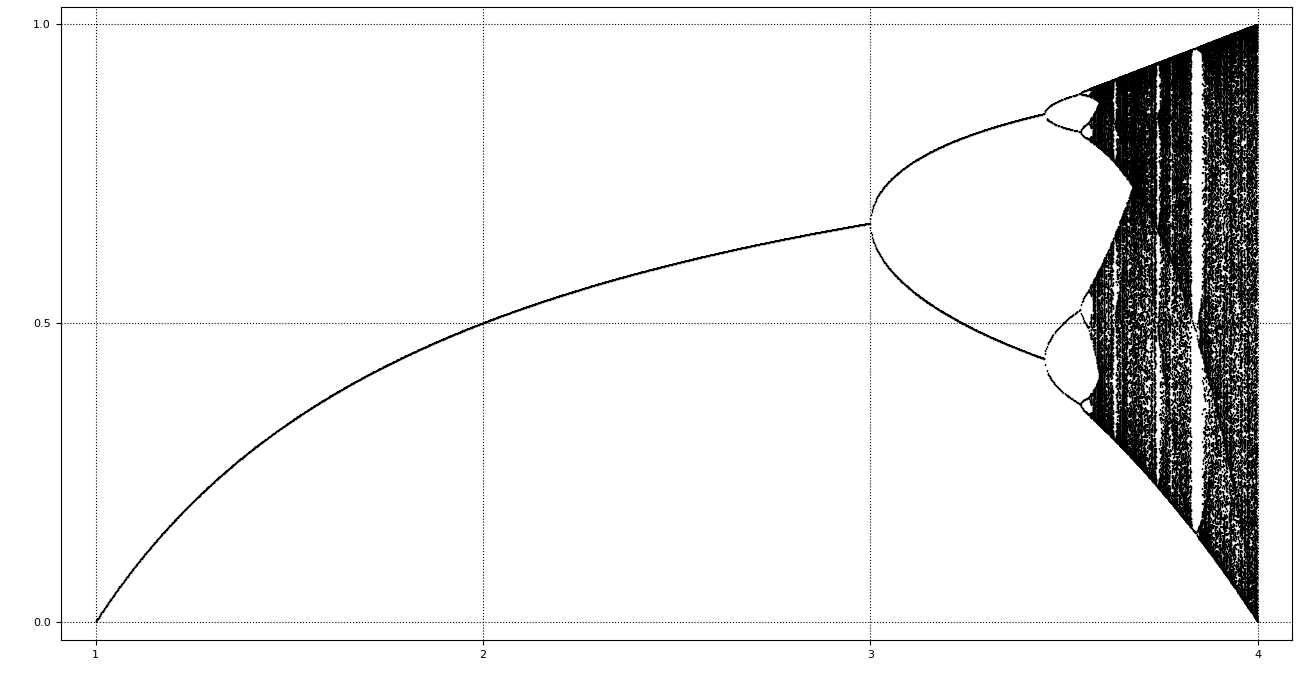
\includegraphics[angle=270,origin=c,height=0.8\textheight]{img/Figure_1} \newpage
  \newline
  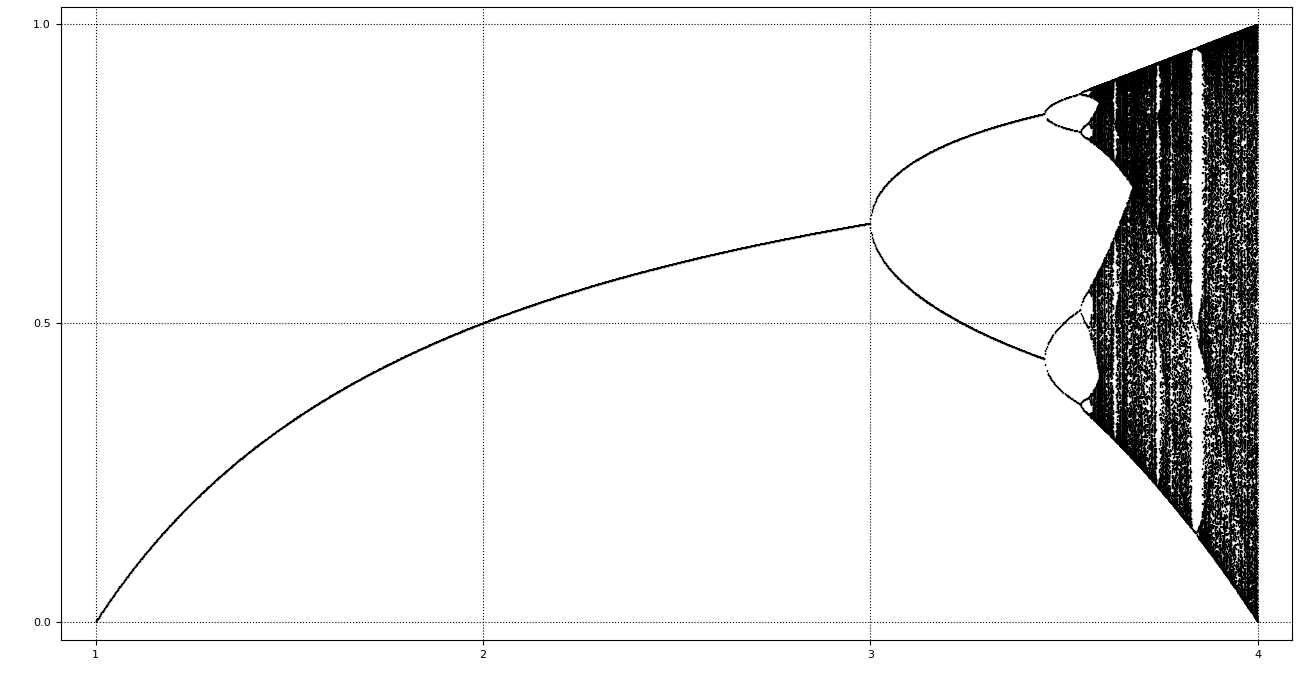
\includegraphics[width=1\textwidth]{img/Figure_1} \newline
  % TODO: dodaj interpretacje
  Dalej podajemy dwie części diagramu dla $x_0 = 0.5$ oraz $r = 4$. \vspace{3mm}\\
  Użyto pojedynczej precyzji:\newline
  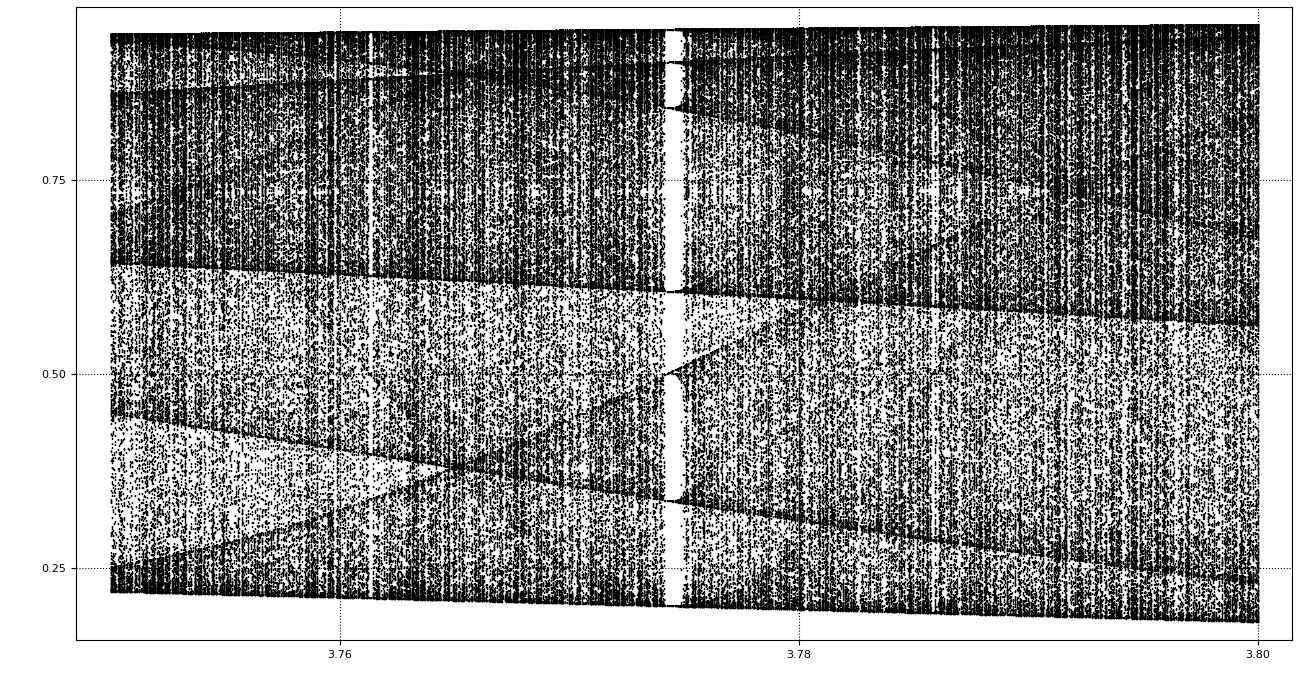
\includegraphics[width=1\textwidth]{img/sp} \newline
  Użyto podwójnej precyzji: \newline
  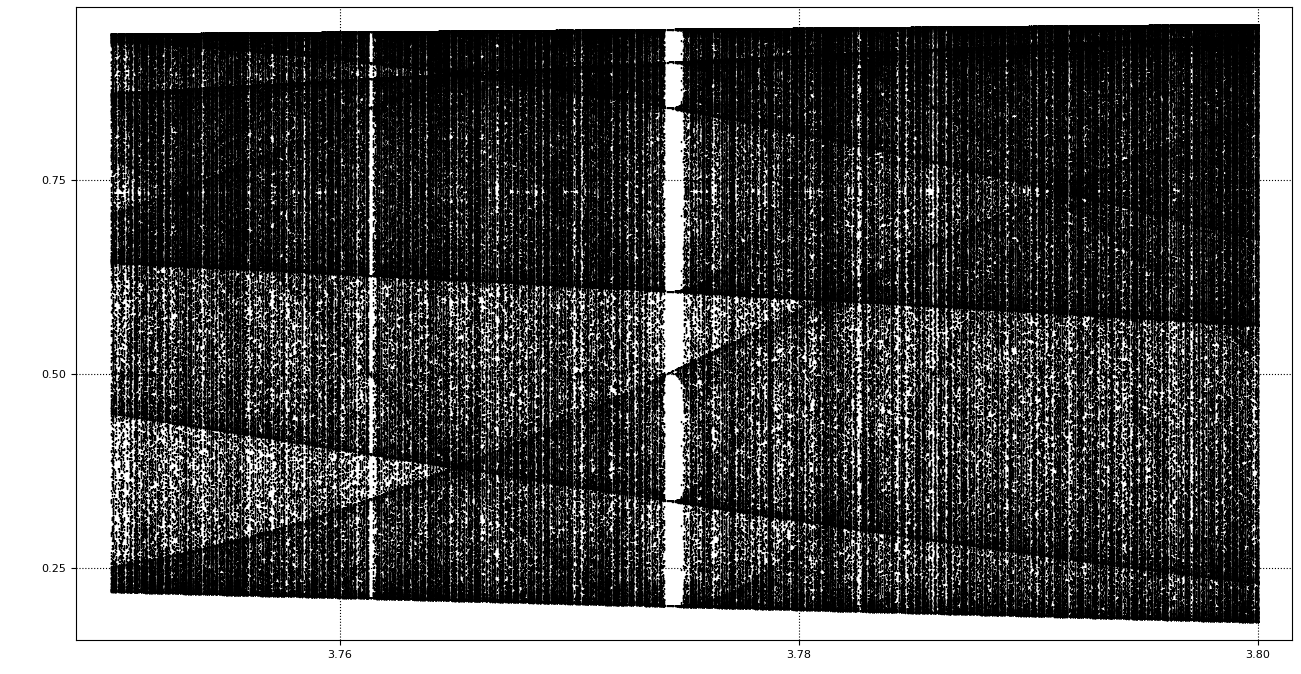
\includegraphics[width=1\textwidth]{img/dp} \newline
  Jak widzimy, diagram, który został wygenerowany przy użyciu podwójnej precyzji
  wygląda 'gęstrzej'. Algorytm, który generuje dany diagram, najpierw szuka
  pierwszego punktu, gdzie funkcja zbieża, a kolejne otrzymuje, porównując do
  już otrzymanych. Kiedy używamy pojedynczej precyzji, nie możemy wykryć
  niektrórych punktów, bo nie możemy rozróżnić dwóch bardzo bliskich siebie
  punktów. Dla tego, używając l.~z. z podwójną precyzją, dostajemy więcej
  punktów. \vspace{3mm}\\
  Liczba iteracji ($n$) potrzebnych do osiągnięcia zera dla $r = 4$ i
  różnych wartości $x_0$: \\
  \begin{tabular}{ | l | l | }
      \hline
      $x_0$ & $n$ \\ \hline
      0.0 & 0 \\ \hline
      0.11111111 & 2659 \\ \hline
      0.22222222 & 5 \\ \hline
      0.33333334 & 2578 \\ \hline
      0.44444445 & 2423 \\ \hline
      0.5555556 & 1306 \\ \hline
      0.6666667 & 2578 \\ \hline
      0.7777778 & 5 \\ \hline
      0.8888889 & 1892 \\ \hline
      1.0 & 1 \\
      \hline
  \end{tabular} % \vspace{3mm}\newline
  % TODO: dodaj interpretacje

\end{document}
\grid
\grid
